\documentclass[a4paper]{article}

%% Language and font encodings
\usepackage[english]{babel}
\usepackage[utf8x]{inputenc}
\usepackage[T1]{fontenc}
\usepackage[section]{placeins}
\usepackage{graphicx}
\usepackage{caption}
\usepackage{subcaption}
\usepackage{float}
\usepackage{verbatim}
\usepackage{color,soul}
\usepackage{indentfirst}
\usepackage{multirow}



%% Sets page size and margins
\usepackage[a4paper,top=3cm,bottom=2cm,left=3cm,right=3cm,marginparwidth=1.75cm]{geometry}

%% Useful packages
\usepackage{amsmath}
\usepackage{graphicx}
\usepackage[colorinlistoftodos]{todonotes}
\usepackage[colorlinks=true, allcolors=blue]{hyperref}
\usepackage{listings}
\usepackage{color} %red, green, blue, yellow, cyan, magenta, black, white
\definecolor{mygreen}{RGB}{28,172,0} % color values Red, Green, Blue
\definecolor{mylilas}{RGB}{170,55,241}
\definecolor{suplightgrey}{rgb}{0.97,0.97,0.94}
% \usepackage[dayofweek]{datetime}
% \newdate{mydate}{26}{04}{2013}
% \usepackage{babel}
\usepackage[useregional]{datetime2}
\DTMsavedate{mydate}{2016-02-10}
\DTMsavedate{date2}{2022-05-26}
% https://mirror.mwt.me/ctan/macros/latex/contrib/datetime2/datetime2.pdf


\title{ECE 44x Project Documentation \\
\large Group: Low Noise and Visibility Drone }

\author{\vspace{2cm} Aaron Jobe \and Evan Newell \and Silas Waxter}
\date{ October 16, 2023}
% \date{\DTMusedate{date2}}

\begin{document}
%\subtitle{Low Noise and Visibility Drone}
\lstset{language=Verilog,%
    backgroundcolor=\color{suplightgrey},
    basicstyle=\small \color{red},
    breaklines=true,%
    keywordstyle=\color{blue},%
    morekeywords=[2]{1}, keywordstyle=[2]{\color{black}},
    identifierstyle=\color{black},%
    stringstyle=\color{mylilas},
    commentstyle=\color{mygreen},%
    showstringspaces=false,%without this there will be a symbol in the places where there is a space
    numbers=left,%
    numberstyle={\tiny \color{black}},% size of the numbers
    numbersep=9pt, % this defines how far the numbers are from the text
    emph=[1]{for,end,break},emphstyle=[1]\color{red}, %some words to emphasise
    captionpos=b,
    %title=\lstname
}

\maketitle
\newpage
\tableofcontents
\newpage

\section{Demonstration of Project}
\hl{see a video of the project at }\href{https://vimeo.com/717762161}{this link}

\section{Project Description}
Summary: This reads data across the PS2 protocol from a keyboard.  It also reads in a background color from switches.  The keyboard keys control a sprite which moves around on a monitor.

Inputs:     PS2 Keyboard, switches.
Outputs:    VGA monitor display

For System Block Diagram, see Figures \ref{fig:sys_bd1} and \ref{fig:sys_bd2}. 

% Project Usage
\vspace{.25 in}
\begin{figure}[h]
  \centering
    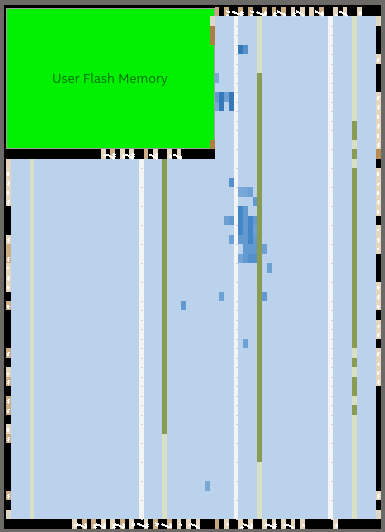
\includegraphics[width=4 in]{Images/project_usage.png}
	\caption{FPGA Usage Displayed}
    \label{fig:keyboard_driver_sim}
\end{figure}
The fully synthesized project uses 1\% of logic elements and 47\% of memory bits.


\newpage
\section{High Level Description}
Figures \ref{fig:sys_bd1} and \ref{fig:sys_bd2} show a block diagram describing the high level functionality of the system.
% System BLock Diagram
\vspace{.25 in}
\begin{figure}[!h]
  \centering
    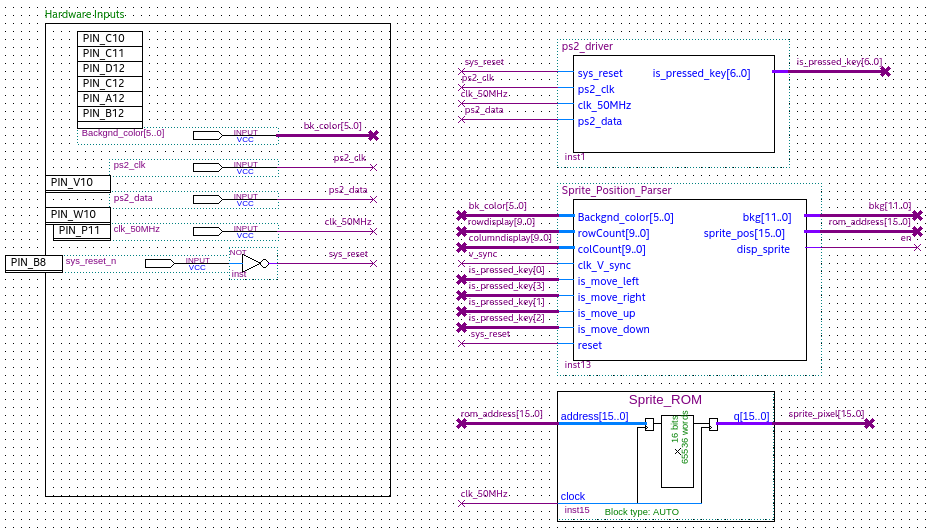
\includegraphics[width=5.91in]{Images/sys_bd_1.png}
	\caption{System Block Diagram Pt. 1}
    \label{fig:sys_bd1}
\end{figure}
\vspace{.25 in}
\begin{figure}[!h]
  \centering
    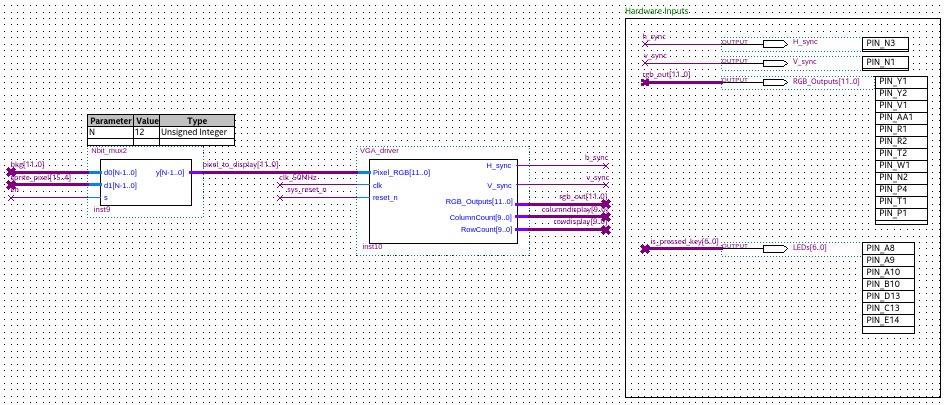
\includegraphics[width=5.91in]{Images/sys_bd_2.png}
	\caption{System Block Diagram Pt. 2}
    \label{fig:sys_bd2}
\end{figure}


\subsection{PS2 Keyboard Driver}
    \hl{Please note that simulation was not run for each block, however integration testing of ps2\_driver proves blocks work as intended.  Furthermore, a block's behaviour can be tested by adding the instantiation of the block within the ps2\_driver as a "wave add ..." command in the ps2\_driver test script}
    \begin{description}
        \item[Summary: ] This driver is responsible for interfacing with the keyboard over the PS2 protocol.  The communication is one-way;  the device (i.e. the keyboard) transmits data which is interpreted by the hose (i.e. the FPGA).  The current implementation exposes the translated keyboard data like a collection of active-high buttons.  The driver mixes polling and event-based techniques.
        \item[Inputs: ] ps2\_clk, ps2\_data, sys\_reset (active-high), clk\_50Mhz
        \item[Outputs: ] is\_pressed\_keys[6..0] is a one-hot active-high bus which encodes which keys are currently being pressed.  The driver internally maps key[0] to 'a', key[1] to 'w', key[2] to 's', and key[3] to 'd'.
    \end{description}
    
    % Block Diagram
    \vspace{.25 in}
    \begin{figure}[h]
      \centering
        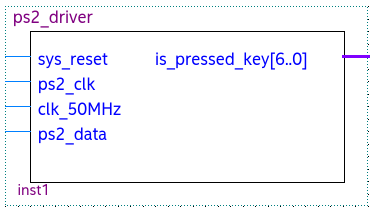
\includegraphics[width=.5\textwidth]{Images/silas_blocks/ps2_driver_bd.png}
    	\caption{PS2 Keyboard Driver, Block Diagram}
        \label{fig:keyboard_driver_bd}
    \end{figure}
    
    % Simulation
    \vspace{.25 in}
    \begin{figure}[h]
      \centering
        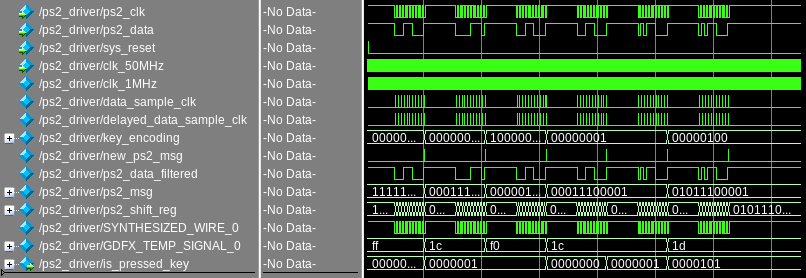
\includegraphics[width=5.91in]{Images/silas_sims/ps2_driver_sim.png}
    	\caption{PS2 Keyboard Driver, Simulation}
        \label{fig:keyboard_driver_sim}
    \end{figure}

    \subsubsection{Filter Register}
        \begin{description}
            \item[Summary: ] The purpose of this register is to prevent any potential glitches or read errors that may occur from sampling the ps2\_data line at one point.  This register samples the signal a parameterized number of times ensuring the value is consistent before updating its output.  Although the block is likely unneeded, it was created when this potential issue was thought to be a primary issue.  The block is still used in the PS2 Keyboard Driver because it makes the driver more robust.
            \item[Inputs: ] reset, input\_to\_filter, sample\_clk
            \item[Outputs: ] filtered\_output
        \end{description}
        
        % Block Diagram
        \vspace{.25 in}
        \begin{figure}[h]
          \centering
            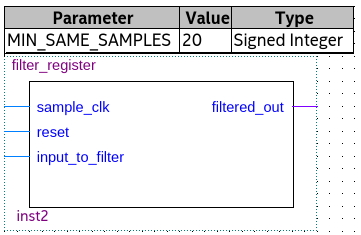
\includegraphics[width=.5\textwidth]{Images/silas_blocks/filter_reg_bd.png}
        	\caption{Filter Register, Block Diagram}
            \label{fig:filter_reg_bd}
        \end{figure}
    \subsubsection{Shift Register}
        \begin{description}
            \item[Summary: ] The purpose of this register is to shift the bits to the left on each rising edge of the clock.  Its useful in parsing ps2\_data into whole messages;  it converts a serial input into a "bussed" output.
            \item[Inputs: ] reset, clk, serial\_in
            \item[Outputs: ] out[N-1:0]
        \end{description}
        
        % Block Diagram
        \vspace{.25 in}
        \begin{figure}[h]
          \centering
            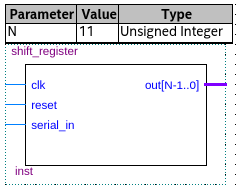
\includegraphics[width=.5\textwidth]{Images/silas_blocks/shift_reg_bd.png}
        	\caption{Shift Register, Block Diagram}
            \label{fig:shift_register_bd}
        \end{figure}
        
        % Simulation
        \vspace{.25 in}
        \begin{figure}[h]
          \centering
            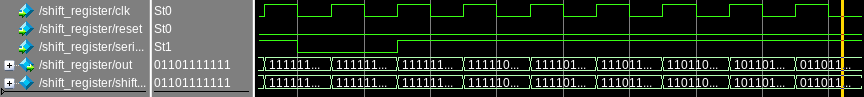
\includegraphics[width=5.91in]{Images/silas_sims/shift_register.png}
        	\caption{Shift Register, Simulation}
            \label{fig:shift_register_sim}
        \end{figure}
    \subsubsection{Hold Register}
        \begin{description}
            \item[Summary: ] This module is used for holding the value from the output of the shift register until a new shift is completed.  The sync\_clk is used to ensure that the completed\_shift is held high for at least one clock cycle;  completed\_shift is used later in the PS2 keyboard driver pipeline for decoding.
            \item[Inputs: ] reset, shift\_clk, sync\_clk, in[N-1:0]
            \item[Outputs: ] out[N-1:0], completed\_shift
        \end{description}
        
        % Block Diagram
        \vspace{.25 in}
        \begin{figure}[h]
          \centering
            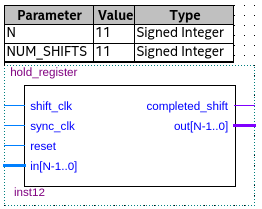
\includegraphics[width=.5\textwidth]{Images/silas_blocks/hold_reg_bd.png}
        	\caption{Hold Register, Block Diagram}
            \label{fig:hold_register_bd}
        \end{figure}
    \subsubsection{Bounded Counter}
        \begin{description}
            \item[Summary: ] This module is used throughout the PS2 keyboard driver.  The bounded counter combines a basic counter with a comparator.  For this module, the parameters are especially important.  N is the number of bits for the counter.  BOUND is the value that sets bound\_reached when the count is equal to it.  IS\_RESET\_ON\_BOUND\_REACHED is a Boolean parameter (1 or 0), and when true (1) the counter will reset itself when the bound is reached;  when false, the counter will keep counting until a reset is triggered on its input or the counter overflows.
            \item[Parameters: ] N, BOUND, IS\_RESET\_ON\_BOUND\_REACHED
            \item[Inputs: ] reset, counted\_signal
            \item[Outputs: ] bound\_reached
        \end{description}
        
        % Block Diagram
        \vspace{.25 in}
        \begin{figure}[h]
          \centering
            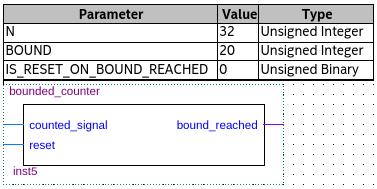
\includegraphics[width=.5\textwidth]{Images/silas_blocks/bounded_counter_bd.png}
        	\caption{Bounded Counter, Block Diagram}
            \label{fig:bounded_coutner_bd}
        \end{figure}
    \subsubsection{Clock Delay Rising Edge}
        \begin{description}
            \item[Summary: ] This module is used to delay a signal;  it was designed for delaying based on a faster signal.  The parameters for this module are important.  NUM\_BIT\_BOUNDED\_COUNTER specifies the number of bits in the bounded counter.  NUM\_FAST\_CLK\_TO\_DELAY specifies the number of clock cycles slow\_clk will be delayed by.
            \item[Parameters: ] NUM\_BIT\_BOUNDED\_COUNTER, NUM\_FAST\_CLK\_TO\_DELAY
            \item[Inputs: ] reset, fast\_clk, slow\_clk
            \item[Outputs: ] delayed\_slow\_clk
        \end{description}
        
        % Block Diagram
        \vspace{.25 in}
        \begin{figure}[h]
          \centering
            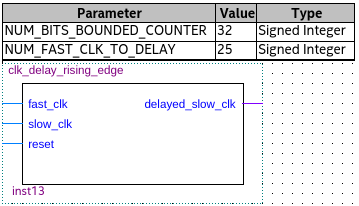
\includegraphics[width=.5\textwidth]{Images/silas_blocks/clk_delay_rising_edge_bd.png}
        	\caption{Clock Delay Rising Edge, Block Diagram}
            \label{fig:clk_delay_rising_edge_bd}
        \end{figure}
        
        % Simulation
        \vspace{.25 in}
        \begin{figure}[h]
          \centering
            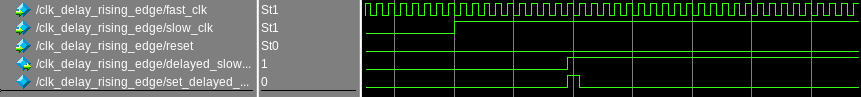
\includegraphics[width=5.91in]{Images/silas_sims/clk_delay_rising_edge.png}
        	\caption{Clock Delay Rising Edge, Simulation}
            \label{fig:clk_delay_rising_edge_sim}
        \end{figure}
    \subsubsection{Button Driver}
        \begin{description}
            \item[Summary: ] This module is used to convert the key codes transmitted by the keyboard into active-high buttons.  There are two kinds of key codes: make codes and break codes (although a break code is really just a release code followed by a make code).  When a button is pressed, the make code of that key is transmitted ("a" transmits 0x1C).  When a button is released, the break code of that key is transmitted ("release a" transmits 0xF0 then 0x1C).  This driver uses polling and events to mimic active-high buttons.  The polling\_clk is connected to a fast clock to reduce the latency the user experiences.  new\_ps2\_msg should signal when a new PS2 message has been passed to the decoder.
            \item[Inputs: ] reset, polling\_clk, new\_ps2\_msg, key\_encoding[7:0]
            \item[Outputs: ] is\_key\_pressed[6:0]
        \end{description}
        
        % Block Diagram
        \vspace{.25 in}
        \begin{figure}[H]
          \centering
            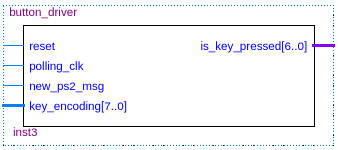
\includegraphics[width=.75\textwidth]{Images/silas_blocks/button_driver_bd.png}
        	\caption{Button Driver, Block Diagram}
            \label{fig:button_driver_bd}
        \end{figure}


\subsection{Sprite\_position\_parser}
\begin{description}
    \item[Summary: ] This block handles the computing and changing of the memory address to make the sprite move around the screen. It is one of the most important blocks that is made up of some simple and some complex modules. This module is expanded and shown in Figure \ref{fig:spriteParses}.
    
    % \item[Inputs: ] clk to be on proper timing should take V\_sync as clock signal, res is an active high asynchronous reset that resets the counter to the lower bound. Pos when activated with logic HIGH will count up with clock rising edge by Pcount amount and the reverse for neg which is counting down.
    
    % \item[Outputs: ] q[N-1:0] is the current count being output from the counter and is used to offset the sprite for movement on the screen.
        
\end{description}

\begin{figure}[H]
    \centering
    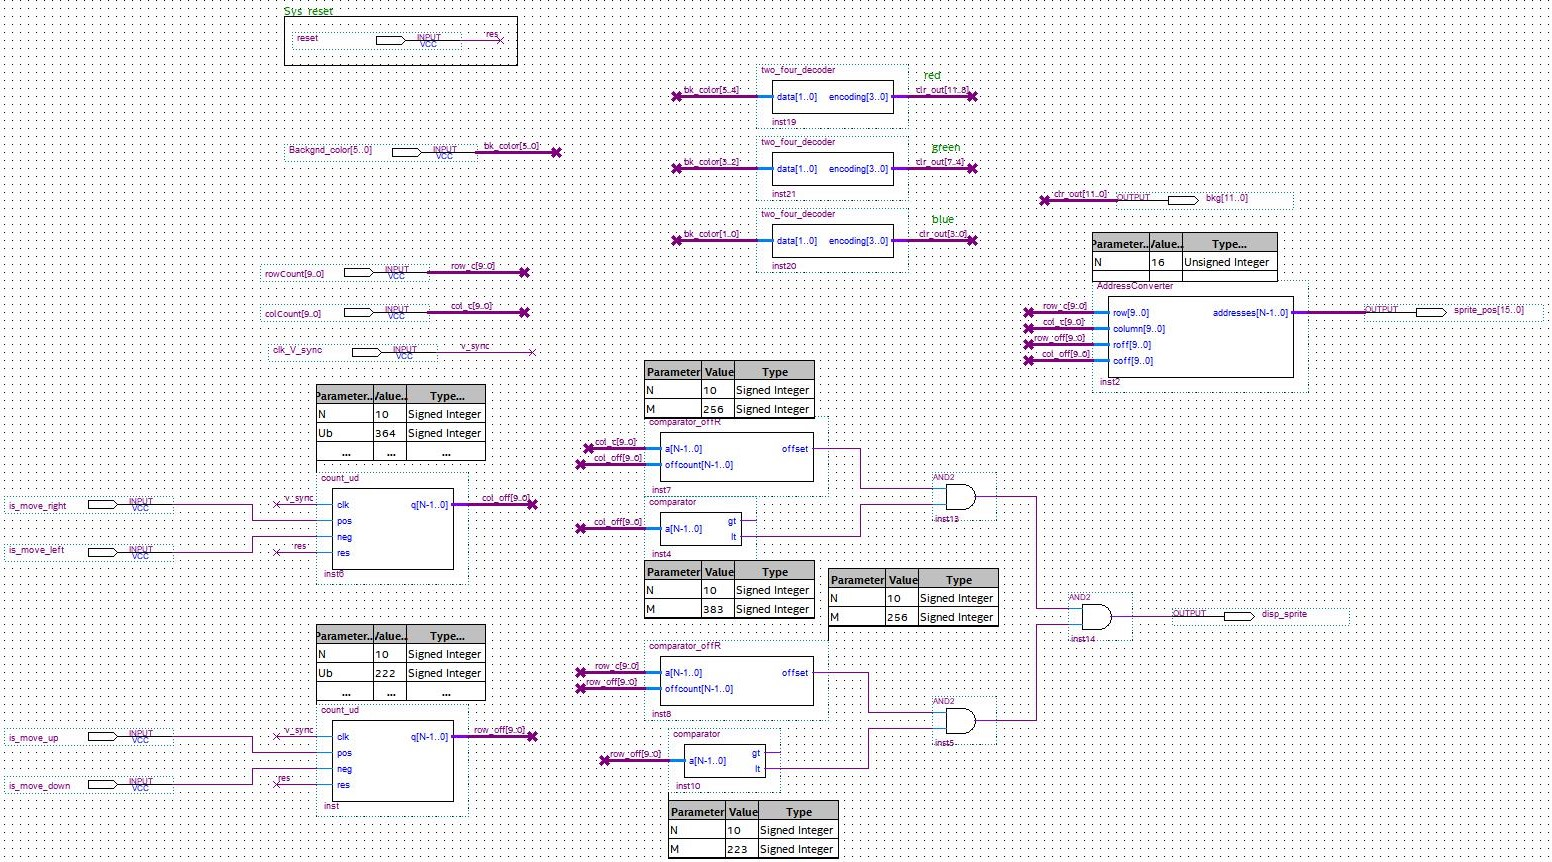
\includegraphics[width=5.9in]{Images/Sprite_Position_Parser.jpg}
    \caption{This block is essential to the movement of the sprite on the monitor through VGA connection.}
    \label{fig:spriteParses}
\end{figure}


\subsubsection{Count\_ud}
\begin{description}
    \item[Summary: ] This bounded counter shown in Figure \ref{fig:count_ud} has an upper and lower bound that it should never go past, when reaching one of the bounds it should stop and stay at that count. This count is used to offset the sprite and move it around the screen. The code for this module is shown in Listing \ref{list:countUD}
    
    \item[Inputs: ] clk to be on proper timing should take V\_sync as clock signal, res is an active high asynchronous reset that resets the counter to the lower bound. Pos when activated with logic HIGH will count up with clock rising edge by Pcount amount and the reverse for neg which is counting down.
    
    \item[Outputs: ] q[N-1:0] is the current count being output from the counter and is used to offset the sprite for movement on the screen.
    
\end{description}

\begin{figure}[H]
    \centering
    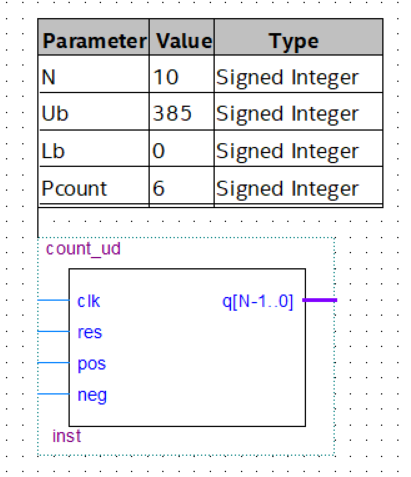
\includegraphics[width=.5\textwidth]{Images/matthew_blocks/countUD.png}
    \caption{This block has many parameters and inputs in order to have the desired effect of being able to increase and decrease the offset of the sprite.}
    \label{fig:count_ud}
\end{figure}

\begin{figure}[H]
    \centering
    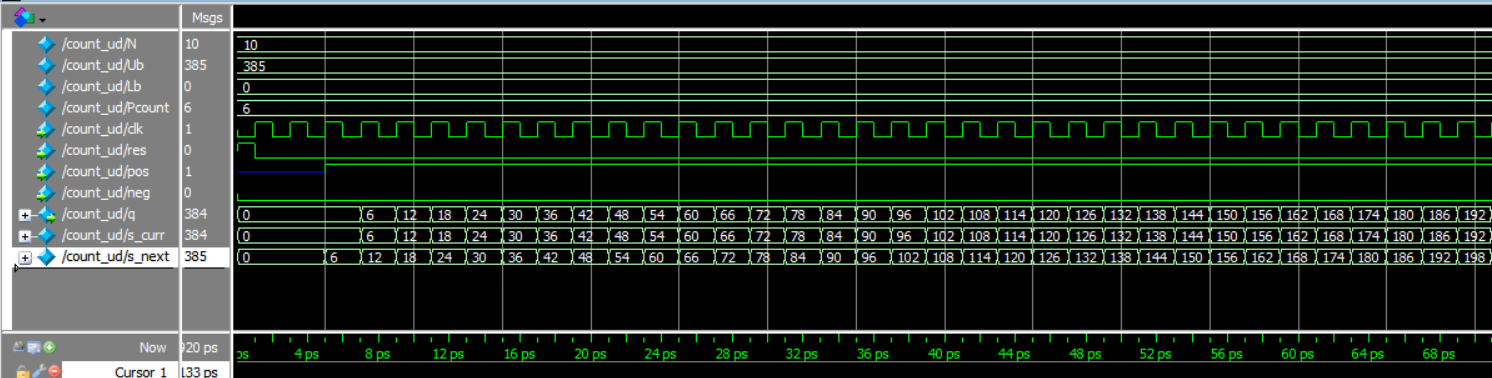
\includegraphics[width=5.91in]{Images/matthew_blocks/countUDSim1.png}
    \caption{This image shows proper counting increments and next state logic in simulation.}
    \label{fig:count_udS1}
\end{figure}

\begin{figure}[H]
    \centering
    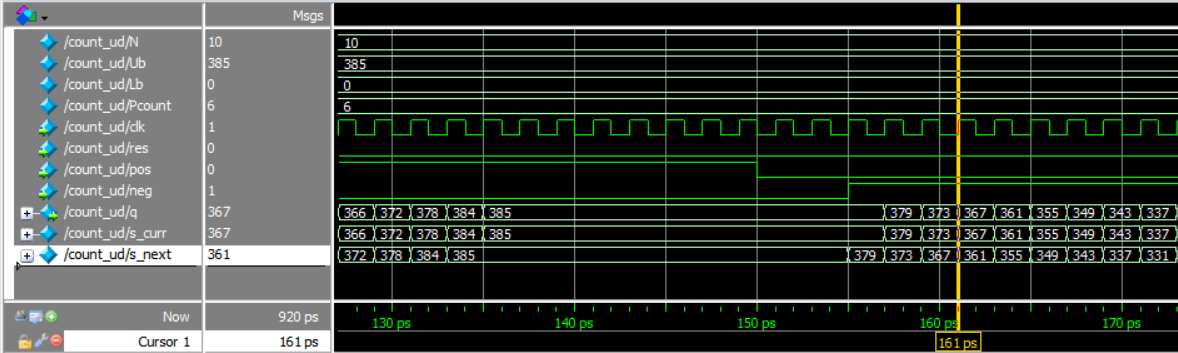
\includegraphics[width=5.91in]{Images/matthew_blocks/countUDSim2.png}
    \caption{This image shows the correct upper-bound count and next state logic during simulation.}
    \label{fig:count_udS2}
\end{figure}

\begin{figure}[H]
    \centering
    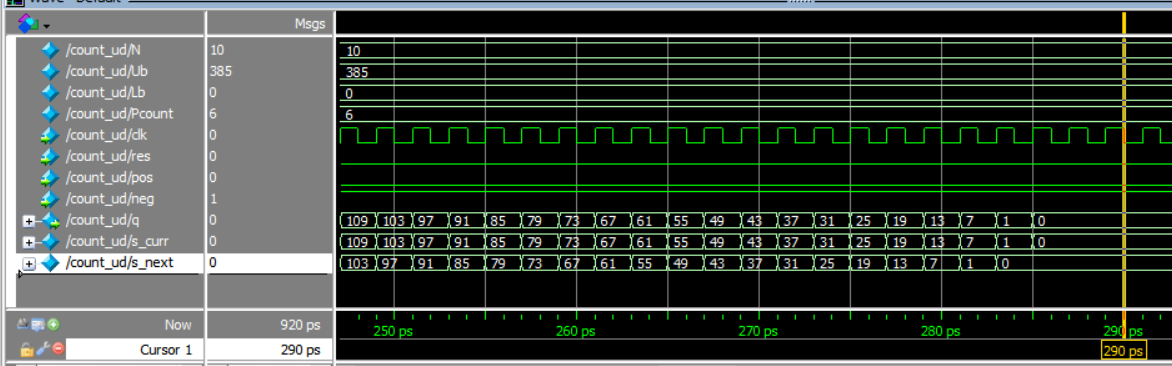
\includegraphics[width=5.91in]{Images/matthew_blocks/countUDSim3.png}
    \caption{This image shows the proper lower-bounding during simulation.}
    \label{fig:count_udS3}
\end{figure}

\subsubsection{Address Converter}
\begin{description}
    \item[Summary: ] The address converter shown in Figure \ref{fig:Address} is a module that calculates which row and column corresponds from the FPGA to how it is stored in the ROM that holds the .mif data which is the sprite. The code for this module is shown in Listing \ref{list:convert}. For convenience the module is based on the equation: $ ((row − roff) \times  ROWVAL) + (column − coff)$.
    
    \item[Inputs: ] row[9:0] is the input for the row count from the VGA\_driver similarly column[9:0] is the input for the column count. roff[9:0] and coff[9:0] are the values to offset row and column by respectively.
    
    \item[Outputs: ] addresses[N-1:0] is the resulting parsed address that goes to the input of the ROM to access the specified address of the provided .mif (sprite data).
\end{description}

\begin{figure}[H]
    \centering
    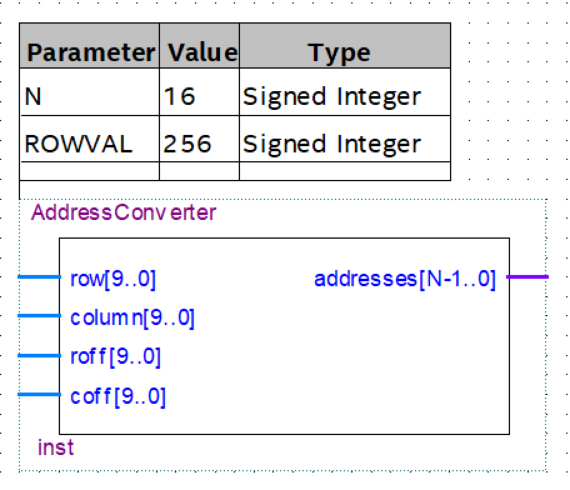
\includegraphics[width=.5\textwidth]{Images/AddressConverter.png}
    \caption{This block calculates the address for the sprite given a specified equation as described earlier and can be seen in Listing \ref{list:convert}}
    \label{fig:Address}
\end{figure}

\begin{figure}[H]
    \centering
    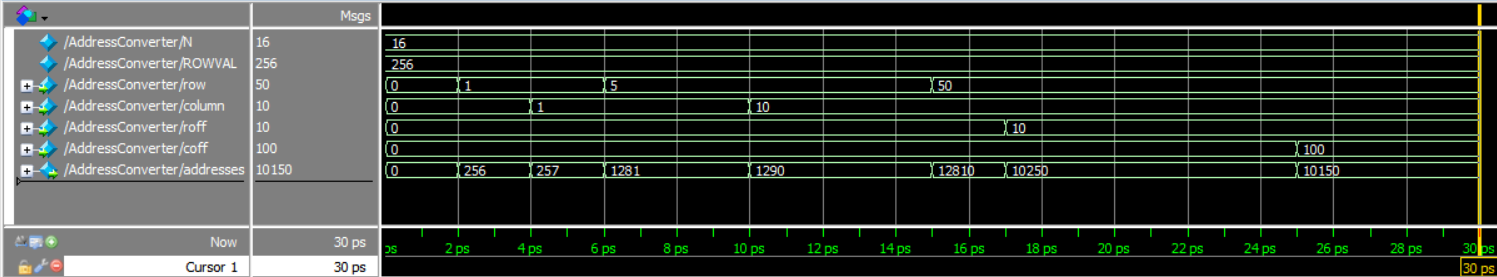
\includegraphics[width=5.91in]{Images/AddressConverterSim.png}
    \caption{This image shows the results of simulation and how the formula behaves.}
    \label{fig:Address_Sim}
\end{figure}

\subsubsection{Comparator\_offR}
\begin{description}
    \item[Summary: ] The comparator shown in Figure \ref{fig:compare_off} is a modified range comparator that constrains a to be greater than or equal to offcount and less than the sum of M and offcount. The purpose of this module is to provide an updating signal of where the sprite is allowed to display on the screen and the naming of the module is to represent that it is a ranged comparator with an offset. The code that represents this module is shown in Listing \ref{list:compareOff}.
    
    \item[Inputs: ] a[N-1:0] is the value compared against the range as described earlier and will take the value of the row or column from the VGA\_driver, offcount[N-1:0] is the value to increase the range offset to aid in the correct display location of the sprite.
    
    \item[Outputs: ] offset is true when a is within the specified range of greater than or equal to the offcount and less than the sum of offcount and parameter M.
\end{description}

\begin{figure}[H]
    \centering
    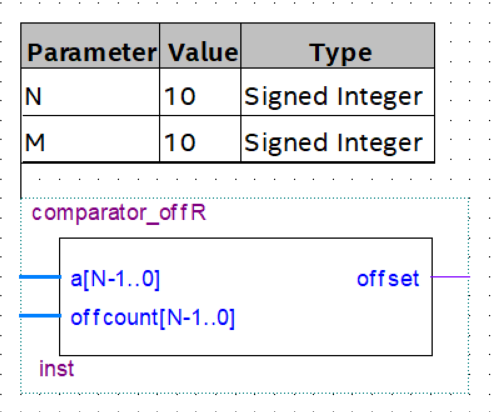
\includegraphics[width=.5\textwidth]{Images/comparator_offR.png}
    \caption{This block is . It is important to note that it handles unsigned integer comparisons more accurately than with signed/negative numbers.}
    \label{fig:compare_off}
\end{figure}

\begin{figure}[H]
    \centering
    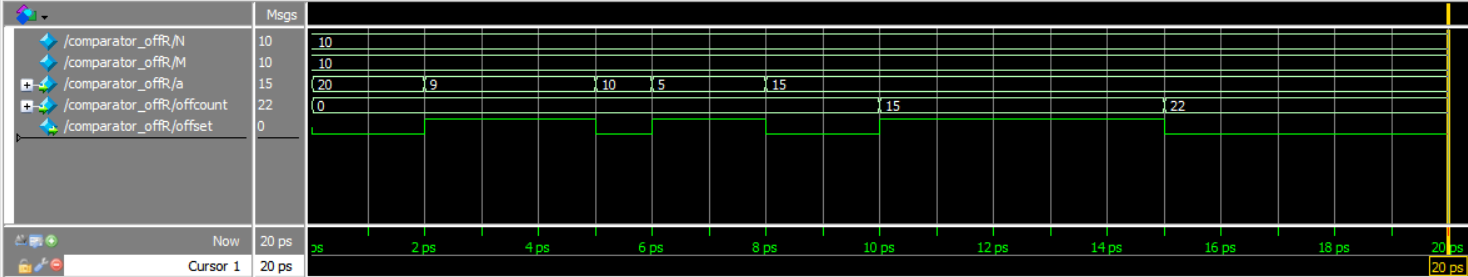
\includegraphics[width=5.91in]{Images/comparator_offR Sim.png}
    \caption{This image shows the proper behavior during simulation.}
    \label{fig:compare_offSim}
\end{figure}

\subsubsection{Two\_four\_decoder}
\begin{description}
    \item[Summary: ] The two to four bit decoder shown in Figure \ref{fig:twofordec} takes a 2-bit input and produces a 4-bit output to make many different combinations of colors with fewer inputs. The code for this module is shown in Listing \ref{list:twofordec}
    
    \item[Inputs: ] data[1:0] 2-bit input that duplicates the 2-bits and adds it to the end making a larger 4-bit number.
    
    \item[Outputs: ] encoding[3:0] the resulting 4-bit number that depends on the input data but it essentially copies the first two bits so 11 would be 1111 or 10 would be 1010 which can be seen by Listing \ref{list:twofordec}
\end{description}

\begin{figure}[H]
    \centering
    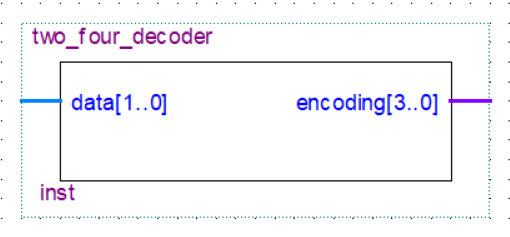
\includegraphics[width=.5\textwidth]{Images/matthew_blocks/twofourdecode.png}
    \caption{This block extends a 2-bit value to 4-bit so more colors can be rendered with less input assignments.}
    \label{fig:twofordec}
\end{figure}

\begin{figure}[H]
    \centering
    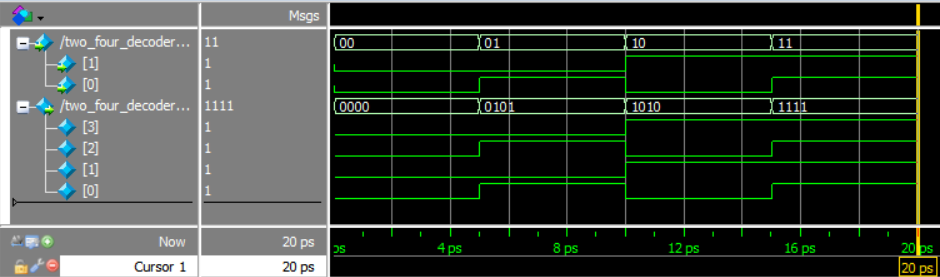
\includegraphics[width=5.91in]{Images/matthew_sim/two_four_decoderSim.png}
    \caption{This simulation shows the proper encoding values.}
    \label{fig:twofordecSim}
\end{figure}

\subsection{VGA\_driver}
\begin{description}
    \item[Summary: ] This block is expanded into a logic diagram shown in Figure \ref{fig:VGA_dBlock} and it handles the proper timings for the 640X480 VGA display that the De10-lite FPGA can handle. It also prepares the colors and H\_sync and V\_sync to be output to the VGA. Finally it does some subtraction on the H\_count and V\_count to get the top left corner of the screen to start displaying the sprite from. The Verilog code that handles how the block operates is shown in Listing \ref{list:VGAdrive}.
    
    \item[Inputs: ] Pixel\_RGB[11:0] are the color bits that are parsed to display at the correct times, the clk runs on a 50MHz clock that it divides in half and it has an active LOW asynchronous reset. The code that represents how this block works is shown in Listing \ref{list:VGAdrive}.
    
    \item[Outputs: ] The H\_sync and V\_sync are output so they can be used when needed and assigned to VGA output pins. RGB\_Outputs[11:0] is the color bits that go to the VGA color pins and RowCount[9:0] and ColumnCount[9:0] determine where the rows and columns of the sprite are parsed to display.
\end{description}

\begin{figure}[H]
    \centering
    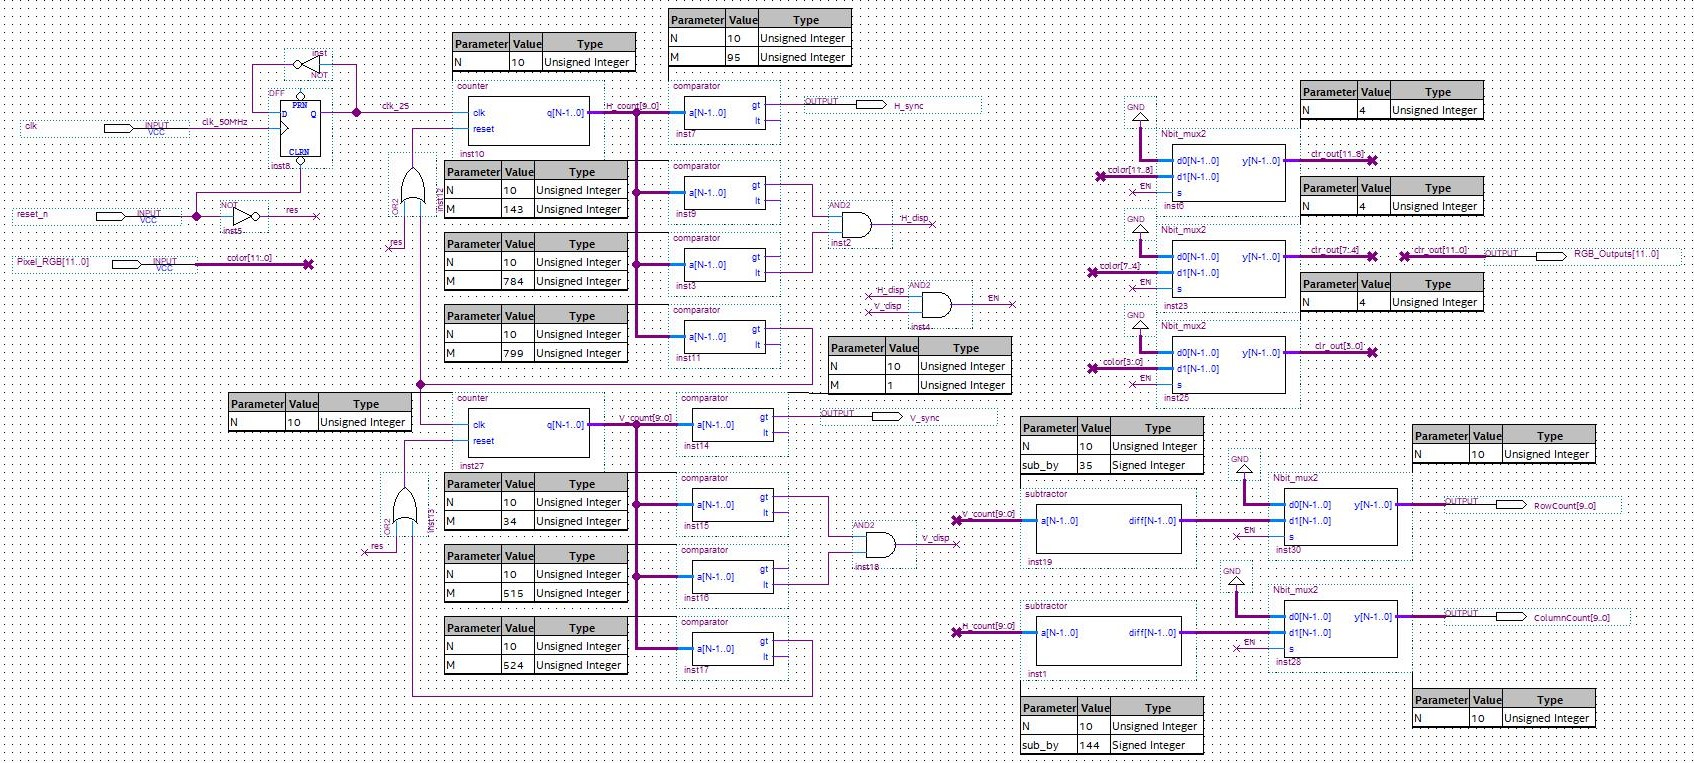
\includegraphics[width=5.91in]{Images/VGA_driver.jpg}
    \caption{This block handles the timings for a 640x480 VGA display for the DE10-Lite FPGA.}
    \label{fig:VGA_dBlock}
\end{figure}

\begin{figure}[H]
    \centering
    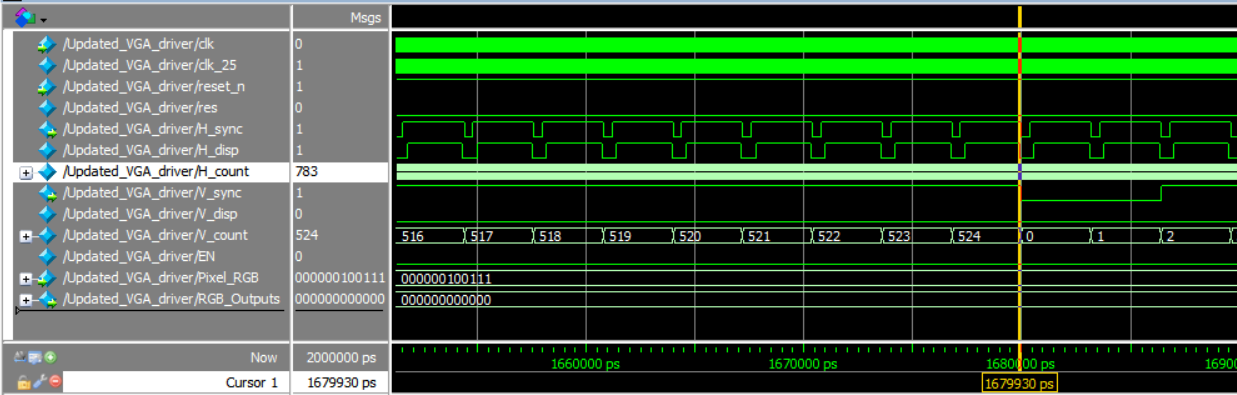
\includegraphics[width=5.91in]{Images/VGA_Driver Proper H_V resets.png}
    \caption{This simulation image shows the proper resetting values for H\_count and H\_sync as well as V\_count and V\_sync.}
    \label{fig:VGAHV_sim}
\end{figure}

\begin{figure}[H]
    \centering
    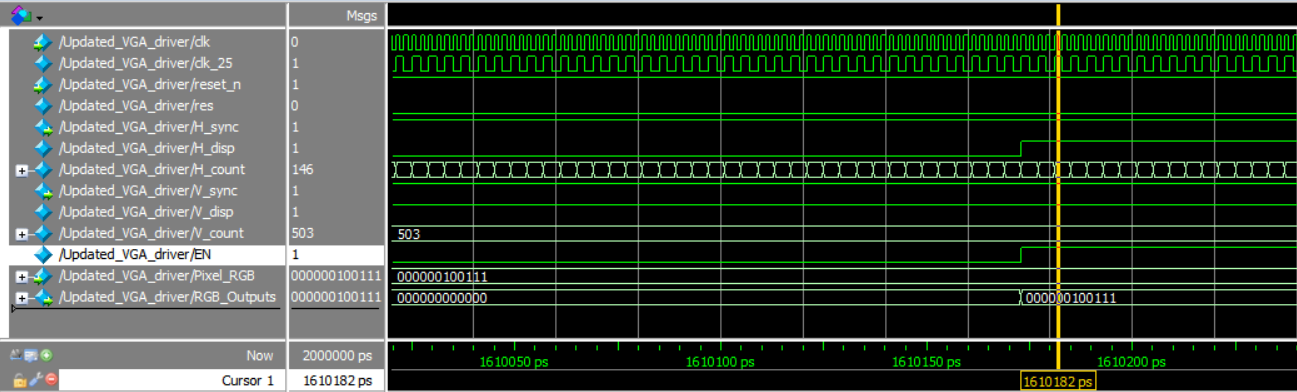
\includegraphics[width=5.91in]{Images/VGA Simulation.png}
    \caption{This image shows a zoomed in view of simulation results.}
    \label{fig:VGA_sim}
\end{figure}

\subsubsection{Counter}
\begin{description}
    \item[Summary: ] The counter shown in Figure \ref{fig:count} is a simple counter with asynchronous reset that is provided in chapter 5 of the text book. The code that represents this module is shown in Listing \ref{list:count}.
    \item[Inputs: ] clk is the signal that works as a clk to increment the counter on a rising edge, reset is an asynchronous reset that will reset the count to 0 anytime an active HIGH value is received.
    \item[Outputs: ] q[N-1:0] is the result of the counter which is incremented on the rising edge of clk.
\end{description}

\begin{figure}[H]
    \centering
    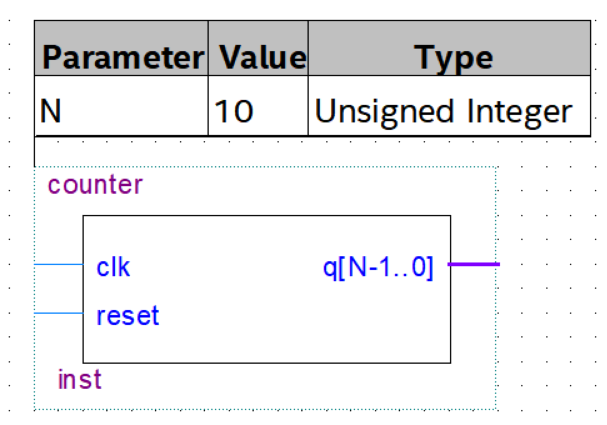
\includegraphics[width=.5\textwidth]{Images/counter.png}
    \caption{This block is modeled after HDL Example 5.5 from chapter 5 of the Digital Design and Computer Architecture textbook.}
    \label{fig:count}
\end{figure}

\begin{figure}[H]
    \centering
    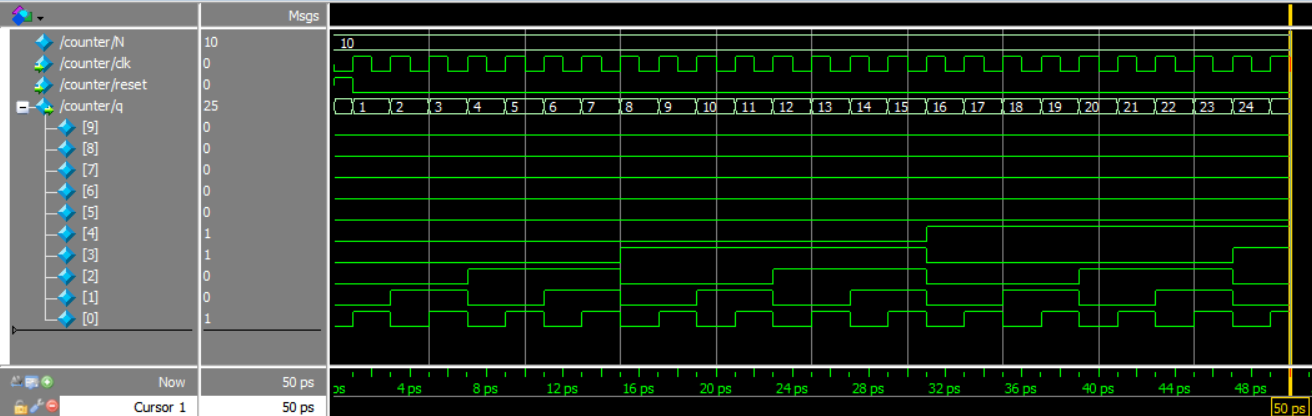
\includegraphics[width=5.91in]{Images/counterSim.png}
    \caption{The simulation results for the counter module.}
    \label{fig:count_sim}
\end{figure}

\subsubsection{Nbit\_mux2}
\begin{description}
    \item[Summary: ] The Nbit\_mux2 shown in Figure \ref{fig:mux2} is a standard 2:1 multiplexer with a variable bit bus for inputs and outputs based off of an example in chapter 4. The code that represents this module is shown in Listing \ref{list:Nmux2}.
    
    \item[Inputs: ] Two parameterized inputs d0[N-1:0], d1[N-1:0] are selected to be output depending on the value of s. If s is 1 then d1's value will be output otherwise d0's will be. 
    
    \item[Outputs: ] y[N-1:0] is the value of d0[N-1:0], or d1[N-1:0] depending on the value of s.
\end{description}

\begin{figure}[H]
    \centering
    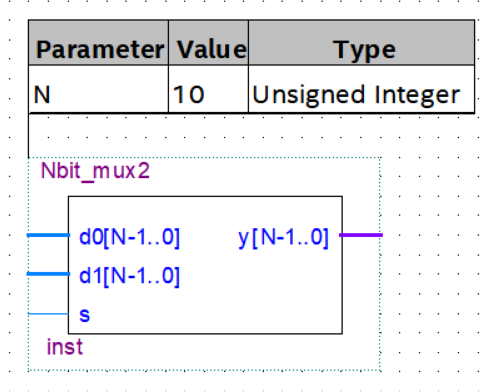
\includegraphics[width=.5\textwidth]{Images/Nbit_mux2.png}
    \caption{This block is modeled after HDL Example 4.5 from chapter 4 of the Digital Design and Computer Architecture textbook.}
    \label{fig:mux2}
\end{figure}

\begin{figure}[H]
    \centering
    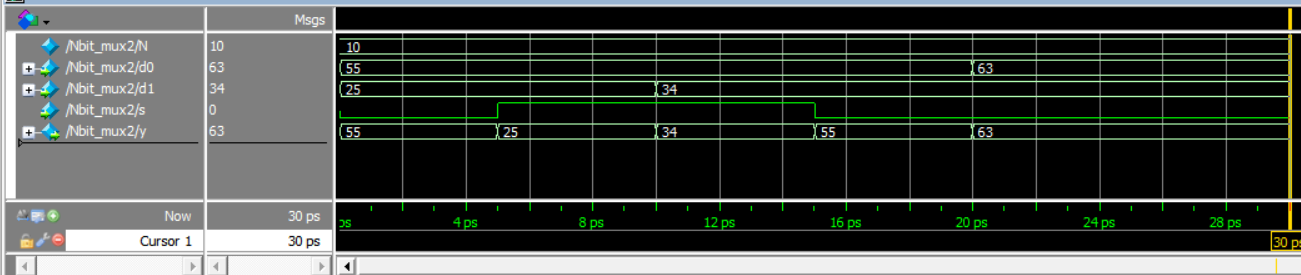
\includegraphics[width=5.91in]{Images/NbitmuxSim.png}
    \caption{The simulation results for the Nbit\_mux2 module.}
    \label{fig:mux_sim}
\end{figure}

\subsubsection{Subtractor}
\begin{description}
    \item[Summary: ] The subtractor shown in Figure \ref{fig:subtractor} is a simple module that subtracts the input value by the provided parameter. The System Verilog code for this module is shown in Listing \ref{list:sub}.
 
    \item[Inputs: ] a[N-1:0] is the value on the right hand side of the subtraction operation and is subtracted from the parameter sub\_by. 
    
    \item[Outputs: ] diff[N-1:0] is the result of the difference between a[N-1:0] and sub\_by.
\end{description}

\begin{figure}[H]
    \centering
    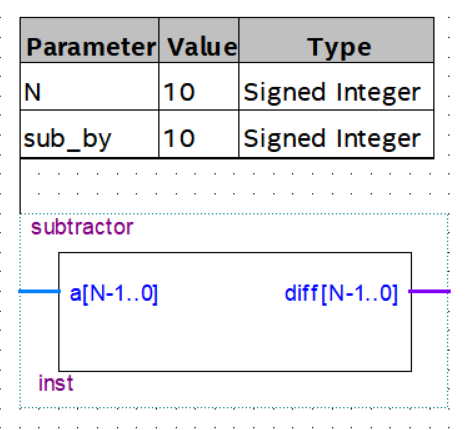
\includegraphics[width=.5\textwidth]{Images/subtractor.png}
    \caption{This block has a simple purpose to subtract off a parameterized value from the input. Note that the type could be changed to unsigned as well.}
    \label{fig:subtractor}
\end{figure}

\begin{figure}[H]
    \centering
    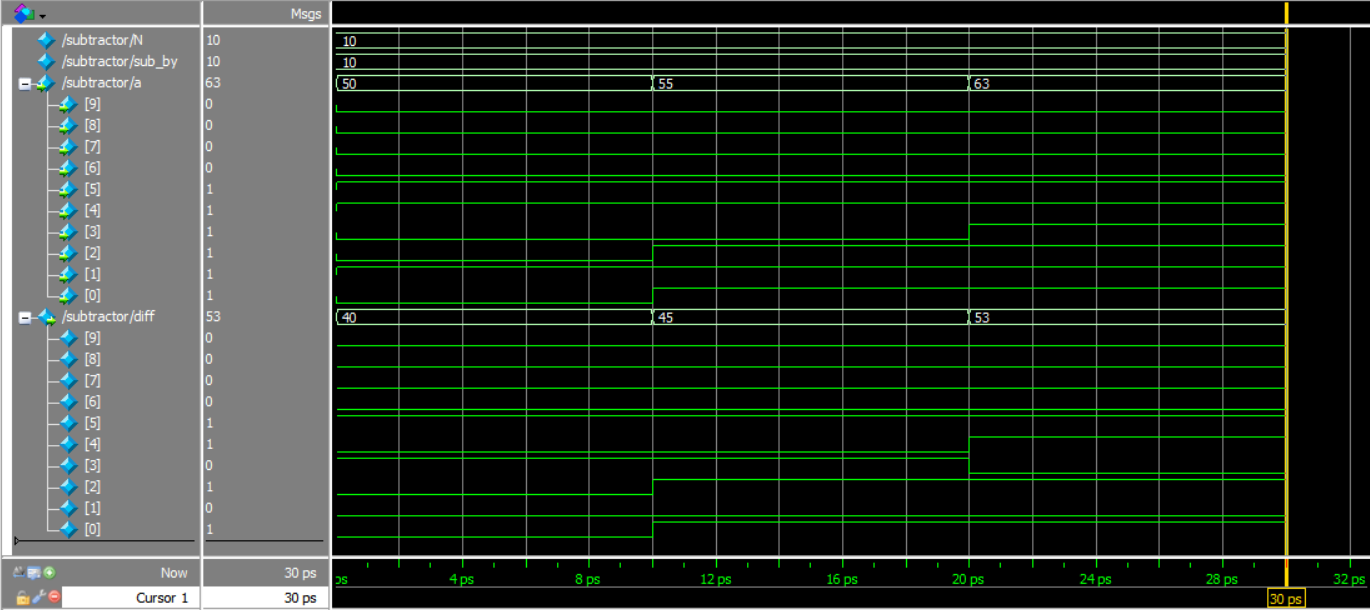
\includegraphics[width=5.91in]{Images/subsim.png}
    \caption{The simulation results for the subtractor module.}
    \label{fig:sub_sim}
\end{figure}

\subsubsection{Comparator}
\begin{description}
    \item[Summary: ] The comparator shown in Figure \ref{fig:compare} is a simple module that compares the input value against the provided parameter. The System Verilog code for this module is shown in Listing \ref{list:compare}.
 
    \item[Inputs: ] a[N-1:0] is the value to be compared against the parameter M.
    
    \item[Outputs: ] gt is active HIGH if a is greater than M otherwise it is LOW, lt is active HIGH if a is less than M other wise it is LOW.
\end{description}

\begin{figure}[H]
    \centering
    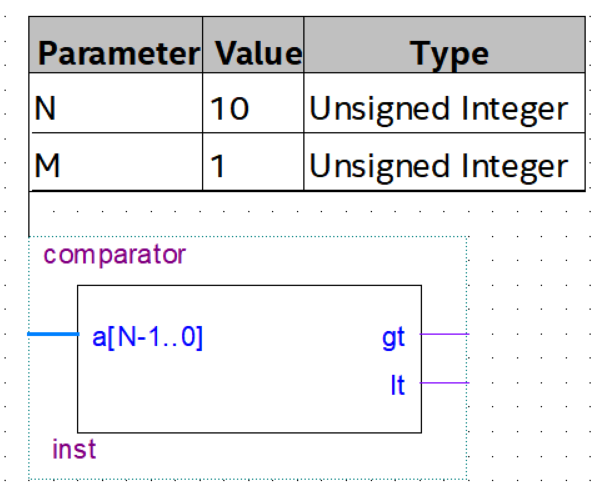
\includegraphics[width=.5\textwidth]{Images/comparator.png}
    \caption{This block has a simple purpose to subtract off a parameterized value from the input. Note that the type could be changed to unsigned as well.}
    \label{fig:compare}
\end{figure}

\begin{figure}[H]
    \centering
    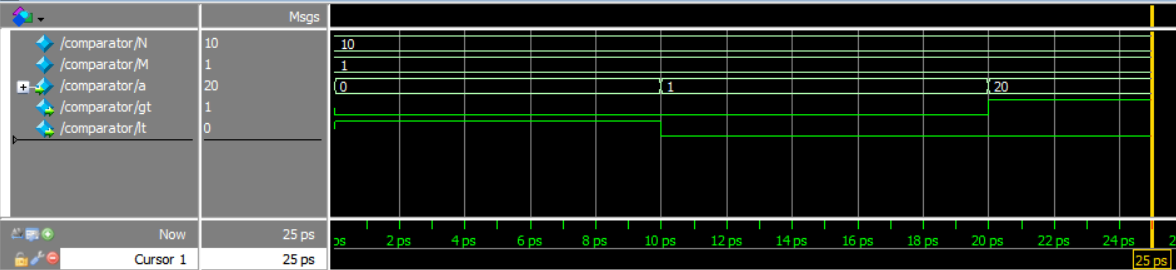
\includegraphics[width=5.91in]{Images/comparatorSim.png}
    \caption{The simulation results for the comparator module.}
    \label{fig:compare_sim}
\end{figure}

\appendix

\section{SystemVerilog Files}
\subsection{PS2 Keyboard Driver}
    \lstinputlisting[caption=PS2 Driver implementation., label=list:ps2imple]{source_files/systemverilog/ps2_driver.v}

    \lstinputlisting[caption=Bounded Counter implementation., label=list:bcimple]{source_files/systemverilog/bounded_counter.sv}
    
    \lstinputlisting[caption=Filter Register implementation., label=list:frimple]{source_files/systemverilog/filter_register.sv}
        
    \lstinputlisting[caption=Shift Register implementation., label=list:srimple]{source_files/systemverilog/shift_register.sv}
        
    \lstinputlisting[caption=Hold Register implementation., label=list:hrimple]{source_files/systemverilog/hold_register.sv}
        
    \lstinputlisting[caption=Button Driver implementation., label=list:bdimple]{source_files/systemverilog/button_driver.sv}
        
    \lstinputlisting[caption=Clock Delay Rising Edge implementation., label=list:cdreimple]{source_files/systemverilog/clk_delay_rising_edge.sv}
        
    \lstinputlisting[caption=Decoder implementation., label=list:dimple]{source_files/systemverilog/decoder.sv}


%Use the lst command to insert the SystemVerilog file, and comment it nicely.
\lstinputlisting[caption=Address converter implementation., label=list:convert]{SystemVerilog/AddressConverter.sv}

\subsubsection{Two\_four\_decoder}
\lstinputlisting[caption=Simple module to extend given bits to make 4-bit output., label=list:twofordec]{SystemVerilog/two_four_decoder.sv}

\subsubsection{Count\_ud}
\lstinputlisting[caption= This complicated System Verilog module is designed to count up and down and be constrained to the given bounds., label=list:countUD]{SystemVerilog/count_ud.sv}

\subsection{VGA\_driver}
\lstinputlisting[caption= The Verilog behind the VGA\_driver block diagram., label=list:VGAdrive]{SystemVerilog/VGA_driver.v}

\subsubsection{Counter}
\lstinputlisting[caption=Simple counter with asynchronous reset implementation., label=list:count]{SystemVerilog/counter.sv}

\subsubsection{Comparator}
\lstinputlisting[caption=Simple comparator with greater than and less than comparisons., label=list:compare]{SystemVerilog/comparator.sv}

\subsubsection{Subtractor}
\lstinputlisting[caption=Simple parameterized subtractor implementation., label=list:sub]{SystemVerilog/subtractor.sv}

\subsubsection{Comparator\_offR}
\lstinputlisting[caption=Ranged comparator with a variable offset input., label=list:compareOff]{SystemVerilog/comparator_offR.sv}

\lstinputlisting[caption=N-bit bus 2:1 multiplexer implementation., label=list:Nmux2]{SystemVerilog/Nbit_mux2.sv}


\lstinputlisting{source_files/systemverilog/keyboard_controlled_sprite.v}

\section{Simulation Files}
\subsection{PS2 Keyboard Driver tcl Scripts}
    \lstinputlisting[caption=tcl file used to simulate ps2\_driver, label=list:ps2\_driver\_tcl]{source_files/simulation_scripts/test_ps2_sample_timing.tcl}
    
    \lstinputlisting[caption=tcl file used to simulate shift\_register, label=list:shift\_register\_tcl]{source_files/simulation_scripts/test_shift_register.tcl}
    
    \lstinputlisting[caption=tcl file used to simulate clk\_delay\_rising\_edge, label=list:clk\_delay\_rising\_edge\_tcl]{source_files/simulation_scripts/test_clk_delay_rising_edge.tcl}
    
\subsubsection{Comparator\_offR macro}
\lstinputlisting[caption=Macro file used to simulate comparator\_offR module., label=list:compareoffdo]{DoFiles/comparator_offR.do}

\subsection{VGA\_driver macro}
\lstinputlisting[caption=Macro file used to simulate VGA\_driver module., label=list:VGAdo]{DoFiles/VGA_Driver.do}

\subsubsection{Counter macro}
\lstinputlisting[caption=Macro file used to simulate counter module., label=list:counterdo]{DoFiles/counter.do}

\subsubsection{Comparator macro}
\lstinputlisting[caption=Macro file used to simulate comparator module., label=list:comparedo]{DoFiles/comparator.do}

\subsubsection{Subtractor macro}
\lstinputlisting[caption=Macro file used to simulate subtractor module., label=list:subdo]{DoFiles/subtractor.do}

\subsection{Sprite\_Position\_Parser macros}
\subsubsection{Count\_ud macro}
\lstinputlisting[caption=Macro file used to simulate count\_ud module., label=list:countupdo]{DoFiles/count_ud.do}

\subsubsection{Nbit\_mux2 macro}
\lstinputlisting[caption=Macro file used to simulate Nbit\_mux2 module., label=list:muxdo]{DoFiles/NbitMux.do}

\subsubsection{AdressConverter macro}
\lstinputlisting[caption=Macro file used to simulate AddressConverter module., label=list:convertdo]{DoFiles/AddressConverter.do}

\subsubsection{Two\_four\_decoder macro}
\lstinputlisting[caption=Macro file used to simulate AddressConverter module., label=list:convertdo]{DoFiles/two_four_decoder.do}



%\bibliographystyle{ieeetr}
%\bibliography{sample}

\end{document}